% !TeX root = ../../main.tex
\section{Zbiory danych}
\label{sec:zbiory}
Do przeprowadzenia eksperymentów (Rozdział \numberref{sec:eksperymenty_wyniki}) skonstruowano dwa zbiory danych, w skład których wchodzą m.in. obrazy otrzymane od firmy \blue{}, wykonane w różnych ośrodkach sportowych.
Jeden zbiór, zwany dalej zbiorem \textit{low}, pochodzi z~kamer sytuowanych na podłodze, tuż przy liniach kortu. Obrazy w zbiorze \textit{low} są monochromatyczne oraz tej samej rozdzielczości.
Drugi zbiór, zwany dalej zbiorem \textit{high} pochodzi z~kamer ustawianych w większej odległości od kortu oraz na wyższej wysokości w porównaniu do zbioru \textit{low}. Zdjęcia w zbiorze \textit{high} są kolorowe i nie charakteryzują się jednakową rozdzielczością.


\begin{figure}[!htb]
  \minipage{0.45\textwidth}
    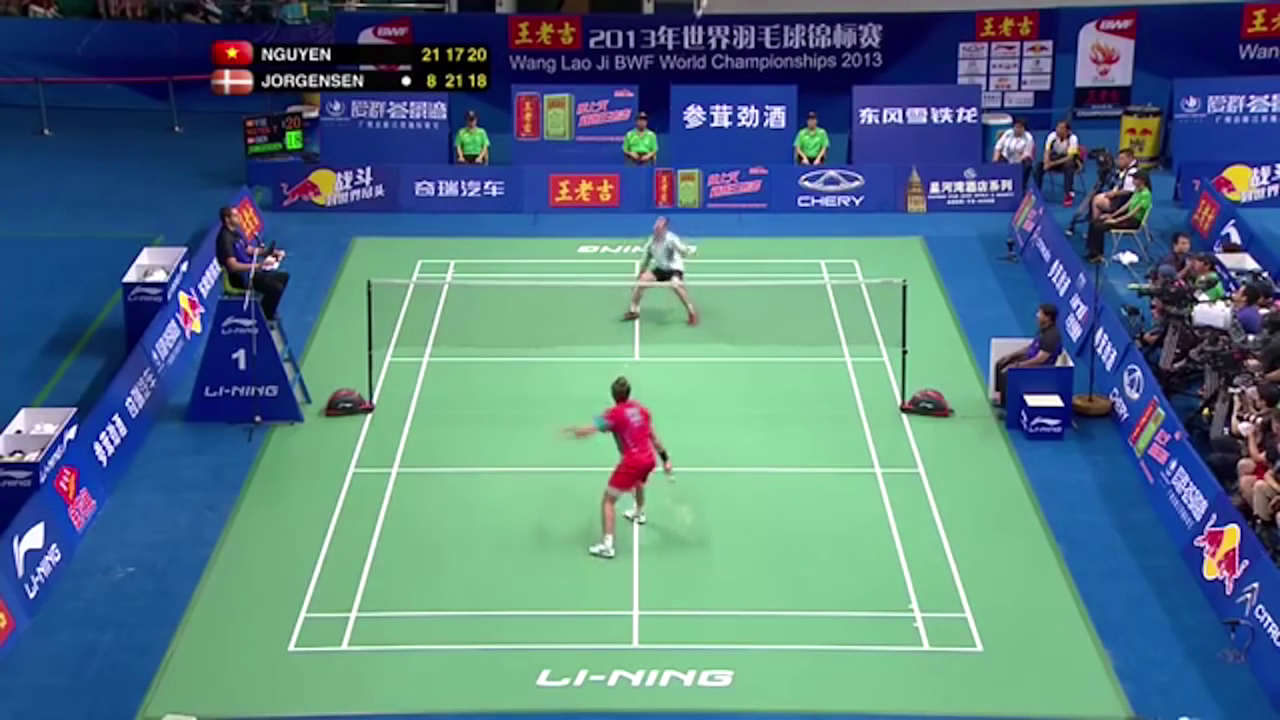
\includegraphics[width=\linewidth]{../../badminton/datasets/high/split/test_court2-00002.png}
    \caption{Przykładowy obraz ze zbioru danych \textit{high} o rozdzielczości 1280x720~pikseli}
  \endminipage\hfill
  \minipage{0.45\textwidth}
    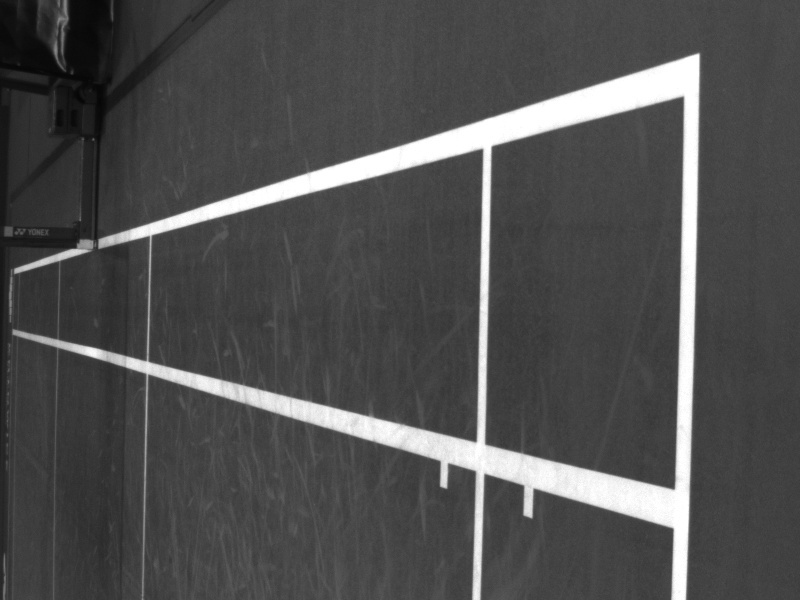
\includegraphics[width=\linewidth]{../../badminton/datasets/low/split/1564909032792410075.jpg}
    \caption{Przykładowy obraz ze zbioru danych \textit{low} o rozdzielczości 896x640~pikseli}
  \endminipage\hfill
\end{figure}

Zbiór \textit{low} zawiera wyłącznie monochromatyczne obrazy o rozdzielczości 896x640 pikseli pozyskane od firmy \blue{}. Obrazy te pochodzą z kamer ustawianych od 50 do 120 centymentrów nad ziemią, w odległości od 75 do 350 centymentrów od najbliższej linii kortu.

\begin{table}[!h]
	\centering
	\caption{Liczność zbiorów danych}
	\vspace{6pt}
	{\footnotesize
		\begin{tabular}{|c|c|c|c|}
			\hline \textbackslash & Liczność \\
      \hline Zbiór \textit{high} & 97 \\
      \hline Zbiór \textit{low} & 207 \\
      \hline
    \end{tabular}
    \label{Tab:licznosc}
	}
	\vspace{0pt}
\end{table}

Zbiór danych \textit{high} składa się z 36 obrazów o wymiarach 1280x720 pikseli, 6 obrazów o rozdzielczości 480x360, 4 obrazów o rozdzielczości 640x480, i pozostałych obrazów o różnych rozdzielczościach, od 259x194 pikseli do 2040x1530 pikseli. Obrazy pochodzą z~różnych źródeł - od firmy \blue{}, z~Internetu (z serwisu \textit{Google Images}) oraz ze~zrzutów ekranu transmisji zawodów sportowych. Sumaryczna liczność elementów w zbiorach danych przedstawiona jest w~tabeli \mytabref{Tab:licznosc}.
